\documentclass[12pt]{extreport}

\usepackage[top=1in,bottom=1.25in,left=1.5in,right=1in]{geometry}
\usepackage{array}
\usepackage{float}
\usepackage{amsfonts}
\usepackage{graphicx}
\usepackage{wrapfig}
\usepackage{setspace}
\usepackage{pgf}
\usepackage{tikz}
\usetikzlibrary{arrows,automata}
\usetikzlibrary{shapes.geometric,fit}
\usepackage{titlesec}
\usepackage{tocloft}
\usepackage{longtable}
\usepackage{lscape}
\usepackage[nottoc]{tocbibind}
\usepackage{fancyhdr}
\usepackage{inputenc}
\usepackage{enumitem}
\usepackage{titlesec}
\usepackage{fixltx2e}
\titleformat{\chapter}[display]
{\normalfont\huge\bfseries\centering}{\chaptertitlename\ \thechapter}{14pt}{\Huge}


\renewcommand{\cftaftertoctitle}{\hrulefill}

\renewcommand*\contentsname{CONTENTS}
\renewcommand*{\listfigurename}{LIST OF FIGURES}
\renewcommand*{\listtablename}{LIST OF TABLES}


\setlist[enumerate,1]{label={(\alph*)}}
\setlist[enumerate,2]{label={(\roman*)}}

\newcounter{parnum}
\newcommand{\N}{%
   \noindent\refstepcounter{parnum}%
    \makebox[\parindent][l]{\textbf{\arabic{parnum}.}}}
    
 \setlength{\parindent}{5em}
    
         
 \renewcommand{\arraystretch}{1.2}  
 
\newcolumntype{M}[1]{>{\centering\arraybackslash}m{#1}} 

\renewcommand{\cfttoctitlefont}{\hspace*{\fill}\Huge\bfseries}
\renewcommand{\cftaftertoctitle}{\hspace*{\fill}}
\renewcommand{\cftlottitlefont}{\hspace*{\fill}\Huge\bfseries}
\renewcommand{\cftafterlottitle}{\hspace*{\fill}}
\renewcommand{\cftloftitlefont}{\hspace*{\fill}\Huge\bfseries}
\renewcommand{\cftafterloftitle}{\hspace*{\fill}}


\begin{document}
%\begin{titlepage}
%\begin{titlepage}
\centering


%\end{document}

%\onehalfspacing
\textbf{A PROJECT REPORT ON}\\\vspace{1cm}\large\textbf{"VOICE CONTROLLED PERSONAL ASSISTANT DEVICE AND CONNECTING IOT DEVICES"}\\\vspace{1cm}

SUBMITTED TO THE SAVITRIBAI PHULE PUNE UNIVERSITY, PUNE
IN THE PARTIAL FULFILLMENT OF THE REQUIREMENTS 
FOR THE AWARD OF THE DEGREE 
\begin{center}

\vspace{1cm} OF\\\vspace{1cm}\textbf{BACHELOR OF ENGINEERING (COMPUTER ENGINEERING) }\\\vspace{1cm}BY\vspace{1cm}\\
{\small{KAPISH KAITH} \hspace{22mm} {\small ROLL NO:13CO028}\\{ROHAN KILLEDAR} \hspace{15mm} {\small ROLL NO:13CO032 } \\{CHAITANYA KULKARNI} \hspace{5mm} {\small ROLL NO:13CO033 } \\{ABHAY DEKATE} \hspace{20mm} {\small ROLL NO:13CO401 }\\\vspace{1cm}}

\end{center}
\textbf{DEPARTMENT OF COMPUTER ENGINEERING}\\ 
\textbf{AISSMS COLLEGE OF ENGINEERING} \\
\begin{center}
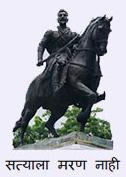
\includegraphics[scale=0.6]{logo.png}
\end{center}
Kennedy Road, Near R.T.O Office, Pune, Maharashtra 411001

2016-2017
\end{titlepage}

%\end{titlepage}

\pagenumbering{roman}
\setcounter{page}{2}
%%\usepackege{setspace}
%\documentclass[letterpaper,12pt]{article}

%\begin{document}
%\fancyput*(x,y){LR stuff }
%\thisfancyput*(x,y){LR stuff }
\noindent
\begin{wrapfigure}{l}{0.2\textwidth}
  \begin{flushleft}
    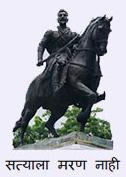
\includegraphics[width=2cm]{logo.png}
  \end{flushleft}
  \end{wrapfigure}
 
	
%\end{document}
\begin {center}

{\LARGE\bf CERTIFICATE}\\\vspace{1.4cm}
\large {This is to certify that the project report entitles}\\\vspace{0.7cm}

{\bf "VOICE CONTROLLED PERSONAL ASSISTANT DEVICE AND CONNECTING IOT DEVICES"}\\\vspace{0.7cm}

\large {Submitted by}\\\vspace{0.5cm}
{\small\bf{KAPISH KAITH} \hspace{36.5mm} {\small ROLL NO:13CO028 } \\{ROHAN KILLEDAR} \hspace{29mm} {\small ROLL NO:13CO032 } \\{CHAITANYA KULKARNI} \hspace{17mm} {\small ROLL NO:13CO033 }\\{ABHAY DEKATE} \hspace{35mm} {\small ROLL NO:13CO401 }}

\end{center}
\vspace{3mm} 

%\paragraph{}
%\begin{flushleft}
\noindent
is a bonafide work carried out by them under the supervision of \textbf{Prof A.M. Jagtap} and it is approved for the partial fulfillment of the requirement of Savitribai Phule Pune University Pune for the award of the degree of Bachelor of Engineering (Computer Engineering) \\

\noindent
This project work has not been earlier submitted to any other Institute or University for the award of any degree or diploma.

%\end{flushleft}


 \vspace{1cm}
 \begin{center}
 
 
\begin{tabular}{c c } 
\bf Prof. N.R. Talhar &\hspace{1cm}\bf Prof. D.P. Gaikwad \\
\bf Guide&\hspace{1cm}\bf Head,\\
\bf Dept. of Computer Engineering &\hspace{1cm} \bf Dept. of Computer Engineering 
\end{tabular}\\
 \end{center}
\vspace{1cm}
\begin{center}
\hspace{10mm}\bf{Dr. S.P. Danao\\\hspace{5mm}Principal\\\hspace{5mm}AISSMS College of Engineering}
\end{center}
\begin{flushleft}
Place : Pune\\
Date  :  
\end{flushleft}

%\pagenumbering{gobble}
\chapter*{\Huge\textbf{ACKNOWLEDGEMENT}}

 We would like to extend my sincere gratitude and thanks to my guide \textbf{Prof. N. R. Talhar}, for his invaluable guidance and for giving us useful inputs and encouragement time and again, which inspired us to work harder.  Due to his forethought, appreciation of the work involved and continuous imparting of useful tips, this report has been successfully completed.\\

\noindent
We are extremely grateful to \textbf{Prof. D.P.Gaikwad}, Head of the Department of Computer Engineering, for his  encouragement during the course of the project work.\\   

\noindent
We also extend our heartfelt gratitude to the staff of Computer Engineering Department for their cooperation and support. \\

\noindent
We also take this opportunity to thank all our classmates,friends and all those who have directly or indirectly provided their overwhelming support during  our project work and the development of this report.\\






\vspace{0.5in}
\begin{tabular}{ll}
 & \hspace{3.5in} \bf Abhay Dekate\\
 & \hspace{3.5in} \bf Chaitanya Kulkarni\\
 & \hspace{3.5in} \bf Rohan Killedar\\
 & \hspace{3.5in} \bf Kapish Kaith\\
\end{tabular}
%\pagenumbering{gobble}

\chapter*{\Huge\textbf{ABSTRACT}}

\hspace*{5em}Crime, nowadays, is increasing as the means to commit them have become more  modernized and opaque in nature.To deal with this new advent, crime analysis needs to be done.Crime 
analysis and prevention is a systematic approach for identifying and analysing patterns and trends in crime. Crime analysis is one of the most important activities  of the majority of 
the intelligent and law enforcement organizations all over the world. Generally the analysis is done by collecting various types of information related to crime or any other event 
significant to those crimes.This information collected can be of any form like audio,images,feeds,alerts,news,text etc.\\

A  major challenge faced by most of the law enforcement and 
intelligence organizations  is efficiently and accurately analysing the growing volumes of related data to crimes and discovering crime patterns and understanding the complex nature 
of the same. Also, nowadays, the diversity and various sources from where such information is generated is vast and dynamic and hence analysis becomes difficult.Data mining is a powerful tool that can be used to analyse such unstructured data effectively and can be used further.\\

The proposed system provides an intelligent and automated way to 
analyse crime news, focusing mainly on crime factors of each day and classify them accordingly.After classification we are going to discover the patterns among the classified data 
and further predict areas or regions prone to crimes so that preventive measures can be taken.If possible will also make an attempt to predict the time frame of the criminal 
activity.This system is going to be a platform oriented  system.



\newpage
\pagestyle{fancy}
\pagenumbering{roman}
\setcounter{page}{4}
\fancyhf{}
\fancyhead[LE,RO]{\textit{\leftmark}}
\fancyhead[RE,LO]{\LaTeX}
\fancyfoot[LE,RO]{\thepage}
\fancyfoot[RE,LO]{\textit{AISSMS COE, PUNE 2015-16}}
 
\renewcommand{\headrulewidth}{2pt}
\renewcommand{\footrulewidth}{1pt}
\newpage

\listoffigures
\newpage
\listoftables
\newpage
\tableofcontents

%%%%%%%%%%%%%%%%%%%% CHAPTER 1 %%%%%%%%%%%%%%%%%%%%%
\chapter{INTRODUCTION}
\pagenumbering{arabic}
\setcounter{page}{1}
\section{BACKGROUND}
\hspace*{5em}India is a vast country with more than one billion population and has a police force of 1.5 million for maintaining law and order to the states and territories, and almost all routine policing, including apprehension of criminals, is carried out by state-level police forces. The police functioning has remained a constant area of governmental concern and efforts to improve it upon further. The Government of India created National Crime Record Bureau (NCRB) in 1986. State Crime Record Bureaux (SCRBx) at States and District Crime Record Bureaux (DCRBx) at Districts were also created to give right impetus to the National Crime Record Bureau.\\


In the background of enormous environmental changes and challenges before the police, harnessing of information became next to impossible. The exchange of information among police agencies became very time consuming and therefore, not available in time of need. There were neither staffs nor time for entering data in records manually. This happened over a period of time all over the country in varying degree. In this scenario, therefore, it became increasingly difficult to coordinate information and come to any meaningful crime analysis. \\


In order to make use of the information technology, Government of India approved the design, development and implementation of a 'Government to Government (G2G), model called the Crime Criminal Information System (CCIS). The CCIS was designed to create computerised storage, analysis and retrieval of crime criminal records. The Crime Criminal Information System today is in operation in all the States. In CCIS, the information is collected at district level not at basic unit of police administration i.e. the police station. Common Integrated Police Application (CIPA) was developed with objective of automation the processes (workflow) at police station and to provide inputs for building CCIS. Till date, CCIS is only collecting the information and creating a huge crime database and there is no analytical tool for analysing huge building database. Absence of crime analysis tool made it somewhat 'standalone' system. Therefore, there is a need of support systems as crime analysis tool based on current technologies to meet and fulfill the new emerging responsibilities and tasks of the Police. 


\section{PROBLEM STATEMENT}
\hspace*{5em}Day by day the crime rate is increasing considerably. Crime cannot be predicted since it is neither systematic nor random. Crime analysis has become one of the most vital activities of the modern world due to the high magnitude of crimes which is a result of technological advancements and the population growth. Law enforcement organizations and the intelligence gathering organizations all around the world usually collect large amounts of domestic and foreign crime data (intelligence) to prevent future attacks. As this involves a large amount of data, manual techniques of analysing such data with a vast variation have resulted in lower productivity and ineffective utilization of manpower. This is one of the most dominant problems in many law enforcement and intelligence organizations. Even though we cannot predict who all may be the victims of crime but can predict the place that has probability for its occurrence.\\

In our current project we are developing a better, efficient crime pattern detection tool to identify crime patterns effectively. It is a supervised learning method in which we are following a sequence of steps : First is Data Collection, second is data classification, third is finding out frequent pattern sets, and last is to predict the crime region where it may take place.\\

In this study we will try to find out more accurate crime prone regions if we consider a particular state/region. We will also try to predict time and happening of crime hotspots.



\section{PURPOSE}
\hspace*{5em}The aim of the project is to identify crime hotspots and predict approximately time of the crime to curb crime in India.


\section{SCOPE}
\hspace*{5em}Predictive mapping promises improvement of  identifying areas in which it focuses interventions as well as improves the way of  implementing it. Thus, helping law enforcers to safeguard and spend their resources wisely, which will effectively improve efficiency as well as bring down the crime rate.






%%%%%%%%%%%%%%%%%%%% CHAPTER 2 %%%%%%%%%%%%%%%%%%%%%
\chapter{LITERATURE SURVEY}

\section{PRESENT WORK} 

\textbf{1. Crime Analysis and Prediction Using Data Mining}\\
\textbf{Authors : Shiju Sathyadevan, Devan M.S and Surya Gangadharan. S}\\\\
Crime analysis and prevention is a systematic approach for identifying and analysing patterns and trends in crime. Our system can predict regions which have high probability for crime occurrence and can visualize crime prone areas. With the increasing advent of computerized systems, crime data analysts can help the Law enforcement officers to speed up the process of solving crimes. Using the concept of data mining we can extract previously unknown, useful information from an unstructured data. Here we have an approach between computer science and criminal justice to develop a data mining procedure that can help solve crimes faster. Instead of focusing on causes of crime occurrence like criminal background of offender, political enmity etc we are focusing mainly on crime factors of each day.\\\\
\textbf{2. Crime Analytics: Analysis of Crimes Through Newspaper Articles}\\
\textbf{Authors : Isuru Jayaweera, Chamath Sajeewa, Sampath Liyanage, Tharindu Wijewardane, Indika Perera and Adeesha Wijayasiri }\\\\
Crime analysis is one of the most important activities of the majority of the intelligent and law enforcement organizations all over the world. Generally they collect domestic and foreign crime related data (intelligence) to prevent future attacks and utilize a limited number of law enforcement resources in an optimum manner. A major challenge faced by most of the law enforcement and intelligence organizations is efficiently and accurately analysing the growing volumes of crime related data. The vast geographical diversity and the complexity of crime patterns have made the analysing and recording of crime data more difficult. Data mining is a powerful tool that can be used effectively for analysing large databases and deriving important analytical results. This paper presents an intelligent crime analysis system which is designed to overcome the above mentioned problems. The proposed system is a web-based system which comprises of crime analysis techniques such as hotspot detection, crime comparison and crime pattern visualization. The proposed system consists of a rich and simplified environment that can be used effectively for processes of crime analysis.\\\\
\textbf{3. Crime Data Mining: A General Framework and Some Examples}\\
\textbf{Authors : Hsinchun Chen Wingyan Chung Jennifer Jie Xu Gang Wang Yi Qin and Michael Chau}\\\\
We conducted a two-hour field study with three Tucson Police Department domain experts who evaluated the analysis' validity by comparing the results against their knowledge of gang organization. They confirmed that the system-found subgroups correctly represented the real groups' organization. For example, the biggest group consisted of gang members involved in many murders and assaults. The second largest group specialized in drug distribution and sales. Interaction patterns between subgroups found in the network were valid as well.\\\\
\textbf{4. Application of NoSQL Database in Web Crawling}\\
\textbf{Authors : GU Yunhua, SHEN Shu, ZHENG Guansheng}\\\\
In this paper the author has explained Web crawling is one of the most important applications of the Internet; the selection of database storage directly affects the performance of search engines. In the past few decades, the traditional relational databases almost monopolize all areas of the database applications. However, with the continuous development of web applications, they are facing the severe challenges. NoSQL database is the broad definition of non-relational data storage.MongoDB supports schema-free, has great query performance with huge amount of data and provides easy horizontal scalability with low cost of hardware. It is more suitable for data storage in Web crawling.Because Mongo DB supports schema-free, we don’t have to design the structure beforehand, and it can be modified at run time. The fields in each document do not need to be same, which can be set depending
on the actual situation when programming.Mongo Db supports embedded document to implement nested, so we can store a post with all the floors in one document that we can efficiently get the whole post by query the id.This article gives the solution of relational
database and NoSQL database MongoDB to meteorological BBS information collection system. The data storage structure and query are designed, and the advantage and the disadvantage are listed in data
structure, query and scalability.\\\\
\newpage
\noindent
\textbf{5. Is Naive Bayes a Good Classifier for Document Classification?}\\\textbf{Authors : S.L. Ting, W.H. Ip, Albert H.C. Tsang}\\\\
In this paper the author has highlighted the performance of implementing Naive Bayes classifier against several other classifiers such as decision tree, neural network, and support vector machines in terms of accuracy and computational efficiency. In their study, Naive Bayes classifier has been discussed as the classifier, which satisfies the literature result. Through their implementation of different feature selection in WEKA tool, they have demonstrated that preprocessing and feature selection are important two steps for improving the mining quality. To test whether Naive Bayes is the best classifier among other classifiers, they have applied three different classifiers for testing. In this experiment, a dataset of 4000 documents are used for evaluation. 1200 documents are extracted randomly to build the training dataset for the classifier. The other 2800 documents are used as the testing dataset to test the classifier. They have summarized that Naive Bayes classifier gave 96.9 percent of accuracy while classifying.\\\\
\textbf{6. Identifying Context of Text Documents using Naive Bayes Classification and Apriori Association Rule Mining}\\
\textbf{Authors : Anagha R Kulkarni, Vrinda Tokekar, Parag Kulkarni }\\\\
They proposed classification of abstracts by considering their context using Naive Bayes classifier and Apriori association rule algorithm - i.e. Context Based Naive Bayesian and Apriori (CBNBA). In proposed approach, they initially classified the documents using Naive Bayes. Ranking these text documents by considering their context will be very useful in information retrieval. They have used Naive Bayes classifier to classify the documents at first level in unstructured format, then found different context of each document by using Apriori-based association rule mining technique to find the words which occur together. They found the context of an abstract by looking for associated terms which helps to understand the focus of the abstract and interpret the information beyond simple keywords. The results indicate that context based classification increases accuracy of classification to great extent and in turn discovers different contexts of the documents. Further this approach can found to be very useful for applications beyond abstract classification where word speaks very little and lead to ambiguous state but context can lead you to right decision/classification.\\\\
\newpage
\noindent
\textbf{7. AN IMPROVED APRIORI ALGORITHM FOR ASSOCIATION RULES}\\
\textbf{Authors : Mohammed Al-Maolegi1, Bassam Arkok2}\\\\
There are several mining algorithms of association rules. One of the most popular algorithms is Apriori that is used to extract frequent itemsets from large database and getting the association rule for discovering the knowledge. Based on this algorithm, this paper indicates the limitation of the original Apriori algorithm of wasting time for scanning the whole database searching on the frequent itemsets, and presents an improvement on Apriori by reducing that wasted time depending on scanning only some transactions. The paper shows by experimental results with several groups of transactions, and with several values of minimum support that applied on the original Apriori and our implemented improved Apriori that our improved Apriori reduces the time consumed by 67.38 percent in comparison with the original Apriori, and makes the Apriori algorithm more efficient and less time consuming.\\\\
\textbf{8. An Implementation of ID3 - Decision Tree Learning Algorithm}\\
\textbf{Authors : Wei Peng, Juhua Chen and Haiping Zhou }\\\\
Decision tree learning algorithm has been successfully used in expert
systems in capturing knowledge. The main task performed in these systems is using inductive methods to the given values of attributes of an unknown object to determine appropriate classification according to decision tree rules. We examine the decision tree learning algorithm ID3 and implement this algorithm using Java programming. We first implement basic ID3 in which we dealt with the target function that has discrete output values. We also extend the domain of ID3 to real-valued output, such as numeric data and discrete outcome rather than simply Boolean value. The Java applet provided at last section offers a simulation of decision-tree learning algorithm in various situations. Some shortcomings are discussed in this project as well.


\section{PROPOSED WORK}
The major goals of our new system are as follows:
\begin{itemize}
\item Predict crime prone regions for a long duration of period
\item Focus on crimes like burglary, pickpocketing ,vehicle theft
,murder,arson etc.
\item Not only will give a criminal profile but also provide a pattern for
similar offences or behaviour of such offenders in multiple other
regions.
\end{itemize}

%%%%%%%%%%%%%%%%%%%% CHAPTER 3 %%%%%%%%%%%%%%%%%%%%%

\chapter{SOFTWARE REQUIREMENTS SPECIFICATION}

\section{INTRODUCTION}
\hspace*{5em}Crime is a human experience and it needs to be controlled.In order to control it effectively, it needs to be analysed perfectly.A major challenge facing all law-enforcement and
intelligence-gathering organizations is accurately
and efficiently analyzing the growing volumes of
crime data. For example, complex conspiracies are
often difficult to unravel because information on
suspects can be geographically diffuse and span long
periods of time. Detecting cyber crime can likewise
be difficult because busy network traffic and frequent
online transactions generate large amounts
of data, only a small portion of which relates to illegal
activities.
Data mining is a powerful tool that enables criminal
investigators who may lack extensive training
as data analysts to explore large databases quickly
and efficiently.Computers can process thousands
of instructions in seconds, saving precious time. In
addition, installing and running software often costs
less than hiring and training personnel. Computers
are also less prone to errors than human investigators,
especially those who work long hours.\\


The main focus of this project is to develop a system that helps to predict the crime pattern and in turn speeds up the process of solving crime and preventing the crime in various regions where system recognizes the pattern.\\
\noindent
\textbf{Objectives:}
\begin{enumerate}
\item To analyse the existing crime analysis and prediction system and identify constraints and problems.

\item To design a new/improved crime analysis and prediction system.
\item To test the new/improved system .
\item To identify conditions for successful implementation of the system. 
\end{enumerate}
     \subsection{PROJECT SCOPE}
\hspace*{5em}The goal is to extract previously unknown, useful information from an unstructured data using the concept of data mining to develop an enhanced data mining procedure that  can help solve crimes faster.Our basic approach attempts to generate a system system that focuses primarily on crime factors of each day for predicting crime prone regions in India over prolonged duration.
     \subsection{USER CLASSES AND CHARACTERISTICS}
\hspace*{5em}This project is meant to offer a brief solution that is faster ,easier,concise and more convenient  than manually analysing the criminal data to predict type of crimes and region where crime is likely to happen.Consequently the application will be able to predict more accurately the crime related data as the usage of system increases that is it gathers or analyses more amount of data related to similar type of crimes.Consequently the user interface will be as intuitive as possible.Also the permissions for accessing the application and features available to all users are same given that they have a valid user credential, as our application will require a user-name and password   to have access due to the nature of application.But the usability for technical expertise that is crime analysts or the general users that is any other law enforcing individual  experience should not be an issue.\\

It is also important that the application be as user friendly as possible, otherwise it will not be a viable alternative for crime analysis 	manually by a crime analyst.Most importantly, the application must be reliable. Regardless of the situation, the application must accurately distribute costs. There is zero tolerance for error when dealing with it as error in such an application may result in inefficient usage of law enforcement resources deployed as per the results given by system for prevention of similar crimes.Thus system accuracy will determine whether the crime analyst wishes to rely on the predicted data or not.

     \subsection{OPERATING ENVIRONMENT}
\hspace*{5em}The main component of our project is the application that we are designing to ease the process of crime analysis and prediction.It is a desktop based system along with requirement of internet connection.The application will require to acquire significant  amount of data from the internet so it requires a decent amount of storage space also it can be used over a network of computers so a standard configuration of the computers over network required.It will not require any cloud support since the whole system will work on an individuals desktop based operating system given that the basic storage requirements is met and we have a good internet connection.The Application Programming Interface (API) required for this software will be built using Java so we require an editor with Java support that is will be needing Java Development  Kit(JDK).Also the algorithms that are going to be implemented in the system will be based on python Implementation.Beyond that, the application is a self-contained unit and will not rely on any other Desktop O.S related software components except for storage space.This software application will be interacting with user at start to determine the source from which user that is crime analyst wishes to gather data for prediction of crime type and region and discover a pattern also at the end for displaying of results as reports generated.While the rest of the time the application will be running itself and there will be no interaction between software and user.The result that is generated in the form of report will be stored either in the database or given as a text file on end user system.Apart form this since the data is stored in Mongo DB  due to its unstructured nature support for Mongo DB and Mongo server will be required.The software application will operate on a network of computers having a internet connection and windows 7/8 or any other new versions as operating system with 4GB of RAM and minimum 1TB of allocated storage space per computer in network of computers.

     \subsection{DESIGN AND IMPLEMENTATION CONSTRAINTS}
\hspace*{5em}The primary design constraint is the Desktop platform. Since the application is designated for Desktop Systems, effective GUI and well user friendliness will be the major design considerations. Creating a user interface which is  both effective and easily navigable is important. Also as we are utilizing the database  for our each of the four major steps based on four different algorithms so storage space need to be considered for smooth functioning of system.Other constraints such as memory and processing power are also worth considering.The analysis and prediction system is meant to be quick and responsive even when dealing with large amount of data so each feature of the software must be designed and implemented considering efficiency.As our system involves four algorithms the system must consider the requirements of all four algorithms for the format of input and output generated and their individual working efficiency and its contribution to overall software applications efficiency.The software will give the desired results only if the specified software requirements are satisfied.\\

At present only Text File format containing data in the form of database records of unstructured data or the algorithm's output format is considered.The system will accept data as input from the database containing unstructured data as records generated by crawling through the web content by a web based crawler and we need active and smooth internet connectivity for effective working of web crawler.\\
Application software designed must implement the algorithms effectively on the collected data and predict the expected result successfully also the interface of software must be easy and simple to be understood by crime analyst and no extra efforts needed by them to understand the usage of software.

\newpage
\noindent
     \subsection{ASSUMPTIONS AND DEPENDENCIES}
     This project will work on the minimum system specifications as follow:
\begin{itemize}
\item Windows 7 or 8 or any other new versions with JDK support.
\item 1TB storage space as HDD.
\item Minimum 4GB ram and i3 processor.
\item Internet connection and smooth access to a network of computers of same physical system configuration.
\item Data stored and accessed from MongoDB an unstructured database that is not SQL.
\end{itemize}
\textbf{Time Dependency:}\\

\noindent
Usability improvements and convenience enhancements that may be added after the application has been developed. Thus, the implementation of these features is entirely dependent upon the time spent designing and implementing the core features. The final decision on whether or not to implement these features will be made during the later stages of the design phase.


%\section{SYSTEM FEATURES}
%This section describes the User interfaces, Hardware interfaces, Software interfaces and Communication interfaces relevant to our project's software application.
\section{EXTERNAL INTERFACE REQUIREMENTS}

 \subsection{USER INTERFACES}
\hspace*{5em}The user interface includes a login window as soon as the application starts with a text box for user-name and a password box for the password.Once the application starts we have normal window consisting of basic menus in title bar, apart from this we have a drop down menu to select the source from where data is to be collected via the web crawler.Also a progress bar depicting the progress of our application as what steps of our algorithm is been completed or being currently executed.A window is provided to display the different attributes on which data was found by the crawler.Another window provided to display the final output that is the predicted crime region and type of crime as well as the pattern identified and matched in that region.
 
 \newpage   
    \subsection{HARDWARE INTERFACES}
The system has following hardware requirements or interfaces:
\begin{itemize}
\item Keyboard:To enter credentials while log in  the system to access it.
\item Mouse:To select the source from drop down menu from which we need to collect data to analyse and predict.
\item Storage:The storage space required to store the collected data as well as output after each stage and the result of the application software in the form of reports.
\item Display Screen:To display the output generated from the application software
\end{itemize}
    
    \subsection{SOFTWARE INTERFACES}
\hspace*{5em}The software interfaces will be the application software developed and the browser used for crawling web data to analyse it further.The browser used is Google chrome which is not operating system dependent.Browser is used to collect input data  and store it in the form of unstructured data in MongoDB with help of web crawler.
    
    \subsection{COMMUNICATION INTERFACES}
\hspace*{5em}A record in the unstructured database stored as a file is used to give input to the crime analysis and prediction system also the communication between various computers on network for achieving concurrent execution is possible via the internet connection working as a communication interface.
    

\section{NON FUNCTIONAL REQUIREMENTS}
\hspace*{5em}These requirements don't affect the system features but play an important role in deciding other factors that are important for a software application to be reliable.
     \subsection{PERFORMANCE REQUIREMENTS}
\hspace*{5em}The system responds to the crime analysts with the predicted crime type and region of crime as per the identified crime patterns as fast as possible  from the time of data collected and stored in database.The time depends upon the time complexity of the Naive Bayes Classifier, Apriori Frequent item-set generation and decision trees.
     \subsection{SAFETY REQUIREMENTS}
\hspace*{5em}The application doesn't affect any other features on machine and since no hardware other than system is used there are no specific safety requirements for handling system.during data collection we have to just take care that system is capable to scale up the storage space so that data is collected without any data loss.
     \subsection{SECURITY REQUIREMENTS}
\hspace*{5em}The application predicts crime patterns and regions so that effectively law enforcement resources can be deployed so that crime can be prevented or avoided.Since this is a very important task as it relates to the security and safety of citizens the decision to deploy resources must be from the authorized party only .Thus we are including a authorization module that will verify the credentials of the user before giving access to the system so that the analysed data is not misused and the system is safe from being compromised.     
     \subsection{SOFTWARE QUALITY ATTRIBUTES}
The application software gives justice to important quality attributes such as:
\begin{itemize}
\item \textbf{Flexibility:}\\ Input related to various domains accepted by the system.
\item \textbf{Reliability:}\\ System generates crime report data which includes the expected output as well as the criminal profiling.
\item \textbf{Usability:}\\Provides simple user interface easily accessible by the concerned user.
\item \textbf{Scalability:}\\System can be used for variable data as well as is scalable on multiple systems over same network.
\item \textbf{Security:}\\Secure as the system asks for user's credentials to provide access to system.
\item \textbf{Dependability:}\\Application software is dependable on the online data collection by web crawler.
\end{itemize}     
     
\newpage
\noindent
\section{OTHER REQUIREMENTS}
\hspace*{5em}These are optional requirements which are not of that importance but if included gives an additive advantage to the application software usage.
    \subsection{DATABASE REQUIREMENTS}
\hspace*{5em}Since our application software is going to work with huge amount of unstructured data it will need an unstructured database that is MongoDB one of the NoSQL Database to store such data.Also the output of the system generated in reports can be stored as text documents in such database.So the database must have a dynamic and scalable schema to avoid any constraint during the working of our application system.
    \subsection{INTERNALIZATION REQUIREMENTS}
\hspace*{5em}Since we are going to analyse crime data from various sources and identify the crime patterns as per each region  we will be discovering many patterns and the system must able to save these patterns even if the data from which it was generated is cleaned so that for each new set of data we have crime patterns already discovered thus helping the system to learn and reduce the time for predicting crime region and type of crime and collecting criminal profiles to generate an effective report as output for our application software.
    \subsection{LEGAL REQUIREMENTS}
\hspace*{5em}The system that we are designing is a system to be used by law enforcers so we need to make sure that our system doesn't violate any laws and also it is not accessible to  criminals or any other  unauthorized person.We need to also take care that the system is well secured, not compromised and the data is not in any form distributed over the web, neither the application is available to other people.The other aspect of such requirement is that we need to make sure system is not exploited by anybody or in any form discredited as it will be our responsibility.
    

\section{ANALYSIS MODEL}

     \subsection{DATA FLOW DIAGRAMS}
     
    \begin{figure}[H]
    \centering
  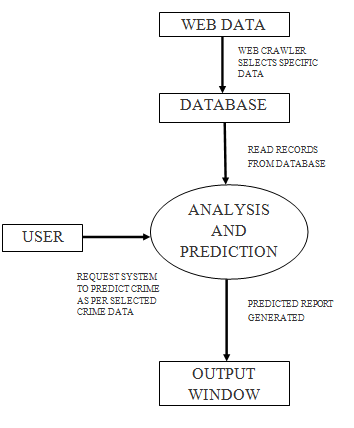
\includegraphics[scale=1.3]{DFDONE.png}\\
  \caption{DFD Level 1}
  
\end{figure}

    \begin{figure}[H]
    \centering
  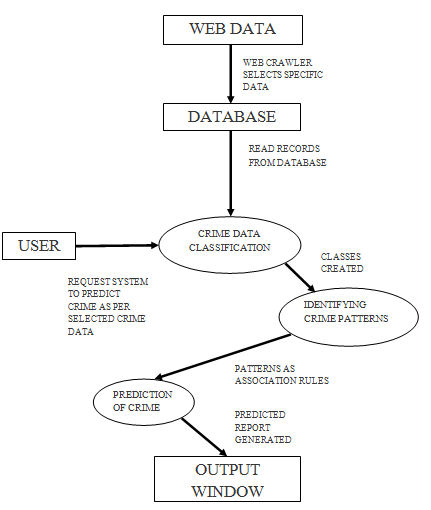
\includegraphics[scale=1.2]{DFDTWO.png}\\
  \caption{DFD Level 2}
  
\end{figure}
   %  \subsection{ENTITY RELATIONSHIP DIAGRAMS}
     \pagebreak
     \subsection{MATHEMATICAL MODEL}
     Let the proposed system be defined by set theory as:\\\\
S= $\{CLA , DC , PRED , PI , S , F , O , I , Q , q_0 , q_f , NDD , D , ALGO \}$ \\ \\
Where, \\ \\
I = input : $\{$ articles, news data, web news data$\}$ \\ \\
O = output :$\{ $type of crime and region as a tuple data$\}$ \\\\
$q_0$ = initial state: $\{$system starts and displays login screen$\}$ \\\\
$q_f$ = final state: $\{$system displays the expected output to user$\}$ \\\\
S = success :$\{$ If the system works accurately without any halt or error.$\}$ \\\\
F = failure :$\{$System halts due to some error or doesn't predict accurately.$\}$\\\\
Q = set of states:$ \{q_0, q_1, q_2, q_3, q_4, q_f\} $\\\\
D = deterministic data : $\{ Null\}$ \\\\
NDD = non deterministic data :$\{$ All states resulting output is non deterministic$\}$\\\\
CLA = classification : $\{ q_2:$ results in classified states or attributes of classes. $\}$\\\\
DC = data collection :$\{ q_1:$ results in data stored in Mongo Db $\}$\\\\
PRED = prediction: $\{q_4:$ results in expected output$\}$\\\\
PI = pattern identification :$\{ q_3:$ results in patterns as association rules$\}$ \\\\
\noindent
\textbf{Naive Bayes Time Complexity : }\\

The complexity of computing the parameters is  
$\Theta(\mid C \mid \mid V\mid)$ because the set of parameters consists of $\mid C \mid \mid V\mid$ conditional probabilities and $\mid C \mid$ priors. The preprocessing necessary for computing the parameters (extracting the vocabulary, counting terms, etc.) can be done in one pass through the training data. The time complexity of this component is therefore $\Theta(\mid D \mid L_{ave})$, where $\mid D \mid$ is the number of documents and $ L_{ave}$ is the average length of a document.\\

\newpage
\textit{Table 3.1} summarizes the time complexities. In general, we have\\
$\mid C \mid \mid V\mid < \mid D \mid L_{ave}$, so both training and testing complexity are linear in the time it takes to scan the data.  $ L_{a}$ and $ M_{a}$ are the numbers of tokens and types, respectively. Because we have to look at the data at least once, NB can be said to have optimal time complexity. Its efficiency is one reason why NB is a popular text classification method.\\

\begin{table}[ht]
\caption{Training \& Testing times for Naive Bayes}
\centering
\begin{tabular}{ |M{4cm}|p{7cm}|  }
 \hline
 mode & time complexity \\
 \hline
 training & $\Theta(\mid D \mid L_{ave} + \mid C \mid \mid V \mid)$\\
 \hline 
 testing & $\Theta(L_{a} + \mid C \mid M_a)=\Theta(\mid C \mid M_a)$\\
 \hline
 
 \end{tabular}

\end{table}
\vspace*{1cm}
\noindent
\textbf{Apriori Algorithm Time Complexity:}\\

Suppose the number of input transactions is N, the threshold is M, number of unique elements is R. The complexity for generating set of size i is $O(R\textsuperscript{$\wedge$}i)$ and the time for calculating support for each set can be done in O(n), if using HashMap. Therefore,  time complexity would be\\
\begin{center}
$O[(R + N) + (R\textsuperscript{$\wedge$}2 + N)  + (R\textsuperscript{$\wedge$}3 + N)  …] $\\
$= O[MN + (R\textsuperscript{$\wedge$}1+R\textsuperscript{$\wedge$}2+ … R\textsuperscript{$\wedge$}M)] $\\
$= O(MN+ (1-R\textsuperscript{$\wedge$}M)/(1-R))$
\end{center}


  \newpage

\section{SYSTEM IMPLEMENTATION PLAN}

\begin{table}[ht]
\caption{System Implementation Plan Phase-I}
\begin{tabular}{ |M{2cm}|p{7cm}|M{2.5cm}|M{3.2cm}|  }
 \hline
 \textbf{SR. NO.} & \textbf{TASK NAME} & \textbf{DURATION} & \textbf{COMPLETION}\\
 \hline
 


  1. & Project Topic Selection &  15 days & $\checkmark$\\
  \hline
  2. & Literature Survey&  10 days& $\checkmark$\\
  \hline
  3. & Study Of Existing System  &  5 days & $\checkmark$\\
  \hline
  4. & Synopsis \& Abstract Submission  &  15 days & $\checkmark$\\
  \hline
   5. & SRS   &  15 days & $\checkmark$\\
   \hline
   6. & Design Of System Architecture &  5 days & $\checkmark$\\
  \hline
  7. & Design Of UML Diagrams  &  5 days & $\checkmark$\\
  \hline
    8. & Planning Of System Modules \& Interface &  8 days & $\checkmark$\\
  \hline
 
  
  
 
 \end{tabular}
 
\end{table}

\begin{table}[ht]
\caption{System Implementation Plan Phase-II}
\begin{tabular}{ |M{2cm}|p{7cm}|M{2.5cm}|M{3cm}|  }
 \hline
 \textbf{SR. NO.} & \textbf{TASK NAME} & \textbf{DURATION} & \textbf{COMPLETION}\\
 \hline
 
 9.& Implementation Of Data Collection \& Storage &	10 Days	& \\
 \hline
 
10. &Implementation Of Classifier &	10 Days	&\\
\hline

11. &Implementation Of Apriori Algorithm	& 10 Days& \\
\hline	
12.&Implementation Of Decision Trees	&10 Days & \\
\hline
13. & Output Display &	8 Days	& \\
\hline
14. & Testing Of Above Modules After Completion of Each Module &	5 Days Per Module	& \\
\hline
15. & Project Review &	5 Days & \\
\hline



 
 \end{tabular}
 
\end{table}


%%%%%%%%%%%%%%%%%%%% CHAPTER 4 %%%%%%%%%%%%%%%%%%%%%

\chapter{SYSTEM DESIGN}

\section{SYSTEM ARCHITECTURE}
The overall system design consists of following modules:
\begin{enumerate}
\item Data Collection.
\item Preprocessing
\item Data Classification.
\item Pattern Identification as frequent item-set.
\item Prediction of Output.

\end{enumerate}
\hspace*{5em}First of all the system starts and ask the user that is crime analyst or the law enforcement authority for credentials to access the system.Then the system proceeds through the credentials verification and the system tasks as shown in the \textit{Figure 4.1} that is the online tasks of system begins by accessing the web content through the web browser with help of web crawler to identify the crime related data specific to the attributes specified then after collection of this data it is stored in an unstructured database MongoDB.After this some preprocessing tasks like cleaning the data stored in database  and formatting it in the form that is suitable for input to the Classifier.
\begin{figure}[H]


	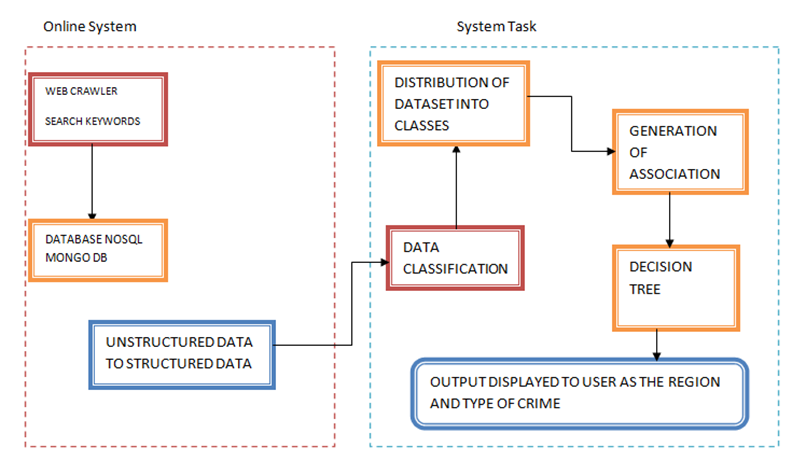
\includegraphics[scale=0.75]{SYSARCH.png}\\
	\caption{System Architecture}
	
	\end{figure}
	The classifier then uses Naive Bayes algorithm for distribution of data collected into classes on basis of attributes like region and type of crime.This is later succeeded by generation of association rules that represent crime patterns and then we analyse or compare various different regions to identify those generated patterns and matching these patterns.Finally we use decision trees to predict the output that is crime region and type of crime, also generates criminal profile which is stored for making the system learn.These all data then accumulated and generated in the form of report to be displayed on screen for the users to decide whether to use that data as per its accuracy or analyse more data.\\
	
The overall flow for the system is shown in \textit{Figure 4.2} that is the  flow  graph for our system.
	\begin{figure}[H]

  \centering
	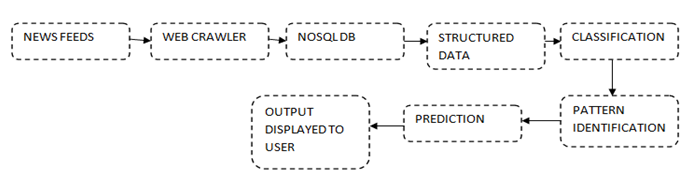
\includegraphics[scale=0.6]{SYSFLOW.png}\\
	\caption{System Flow Graph}
	
	\end{figure}
\section{UML DIAGRAMS}

\section*{\underline{Definition}}
\hspace*{5em}The Unified Modelling Language (UML) is a general purpose,developmental, modelling language in the field of software
engineering, that is intended to provide a standard way to visualize the design of a system. UML was originally motivated by the desire to standardize the disparate notational systems and approaches to software design.


\section*{\underline{Design}}
The Unified Modelling Language (UML) offers a way to visualize a system's architectural blueprints in a diagram  including elements such as:
\begin{itemize}


\item Any activities.
\item Individual components of the system:
And how they can interact with other software components.
\item How the system will run.
\item How entities interact with others (components and interfaces)
\item External user interface
\end{itemize}
\hspace*{5em}Although originally intended solely for object oriented design documentation, the Unified Modelling Language (UML) has been extended to cover a larger set of design documentation.


\section*{\underline{UML System Model}}
\begin{itemize}
\item \textbf{Static (or structural) view:}\\
Emphasizes the static structure of the system using objects, attributes,
operations and relationships. The structural view includes class diagrams and composite structure
diagrams.
\item \textbf{Dynamic (or behavioural) view:}\\
Emphasizes the dynamic behaviour of the system by showing collaborations among objects and changes to the internal states of objects. This view includes sequence diagrams, activity diagrams and state machine diagrams.
\end{itemize}

\section*{\underline{UML Models}}
\begin{enumerate}
\item \textbf{Use case diagram:}\\
To model a system the most important aspect is to capture the dynamic behaviour.
To clarify a bit in details, dynamic behaviour means the behaviour of the system when it is running /operating.
So only static behaviour is not sufficient to model a system rather dynamic
behaviour is more important than static behaviour.These internal and external agents are known as actors. So use case diagrams are consists of actors, use cases and their relationships. The diagram is used to model the system/subsystem of an application. A single use case diagram captures a particular functionality of a system.
So to model the entire system numbers of use case diagrams are used.
\item \textbf{Deployment Diagram:}\\
Deployment diagrams are used to visualize the topology of the physical
components of a system where the software components are deployed.
So deployment diagrams are used to describe the static deployment view of a system. Deployment diagrams consist of nodes and their relationships.
The name Deployment itself describes the purpose of the diagram. Deployment diagrams are used for describing the hardware components where software components are deployed. Component diagrams and deployment diagrams are closely related.
UML is mainly designed to focus on software artefacts of a system. But these two diagrams are special diagrams used to focus on software components and hardware components.So most of the UML diagrams are used to handle logical components but
deployment diagrams are made to focus on hardware topology of a system.
Deployment diagrams are used by the system engineers.
\item \textbf{Activity Diagram:}\\
Activity diagram is basically a flow chart to represent the flow form one activity toanother activity. The activity can be described as an operation of the system.So the control flow is drawn from one operation to another. This flow can be sequential, branched or concurrent. Activity diagrams deals with all type of flow control by using different elements like fork, join etc.
It captures the dynamic behaviour of the system. Other four diagrams are used to show the message flow from one object to another but activity diagram is used to show message flow from one activity to another.
It does not show any message flow from one activity to another. Activity diagram is some time considered as the flow chart. Although the diagrams looks like a flow chart but it is not. It shows different flow like parallel, branched, concurrent and single.

\newpage
\noindent
\item \textbf{Sequence Diagram:}\\
A Sequence diagram is an interaction diagram that shows how processes operate with
one another and in what order. It is a construct of a Message Sequence Chart. A sequence
diagram shows object interactions arranged in time sequence. It depicts the objects
and classes involved in the scenario and the sequence of messages exchanged between
the objects needed to carry out the functionality of the scenario. Sequence diagrams
are typically associated with use case realizations in the
Logical View of the system under development. Sequence diagrams are sometimes called
event diagrams or event scenarios.
A sequence diagram shows, as parallel vertical lines (lifelines), different processes
or objects that live simultaneously, and, as horizontal arrows, the messages exchanged between them, in the order in which they occur. This allows the specification of simple runtime scenarios in a graphical manner.

\item \textbf{State Chart Diagram:}\\
The name of the diagram itself clarifies the purpose of the diagram and other details. It describes different states of a component in a system. The states are specific to a component/object of a system. A State chart diagram describes a state machine. Now to clarify it state machine can be defined as a machine which defines different states of an object and these states are controlled by external or internal events. Activity diagram explained in next chapter, is a special kind of a State chart diagram. As State chart diagram defines states it is used to model lifetime of an object. State chart diagram is one of the five UML diagrams used to model dynamic nature of a system. They define different states of an object during its lifetime. And these states are changed by events. So State chart diagrams are useful to model reactive systems. Reactive systems can be defined as a system that responds to external or internal events. State chart diagram describes the flow of control from one state to another state. States are defined as a condition in which an object exists and it changes when some event is triggered.

\item \textbf{Class Diagram:}\\
In software engineering, a class diagram in the Unified Modelling Language (UML) is a type of
static structure diagram that describes the structure of a system by showing the system's classes, their attributes, operations (or
methods), and the relationships among objects.The class diagram is the main building block of object oriented modelling. It is used both for general
conceptual modelling of the systematics of the application, and for detailed modelling translating the models into programming code. Class diagrams can also be used for data modelling.In the diagram, classes are represented with boxes which contain
three parts as follows the top part contains the name of the class, the middle part contains the attributes of the class and the bottom part contains the methods the class can execute.\\

\end{enumerate}

\pagebreak
    \subsection{USE CASE DIAGRAM}
    \begin{figure}[H]
    \centering
  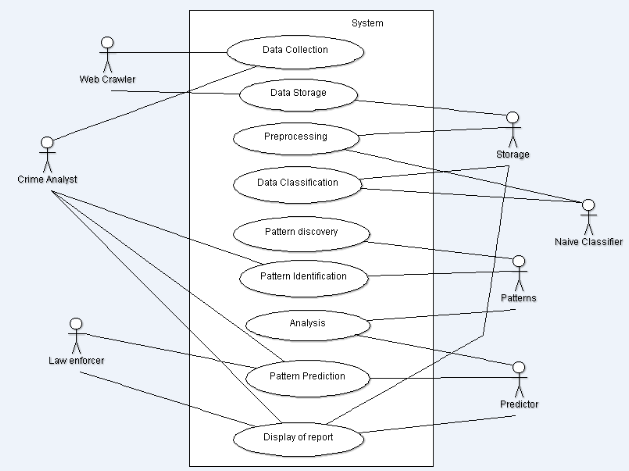
\includegraphics[scale=0.75]{USECRIME.png}\\
  \caption{Use Case Diagram}
  
\end{figure}
    \pagebreak
    \subsection{DEPLOYMENT DIAGRAM}
     \begin{figure}[H]
  \centering
  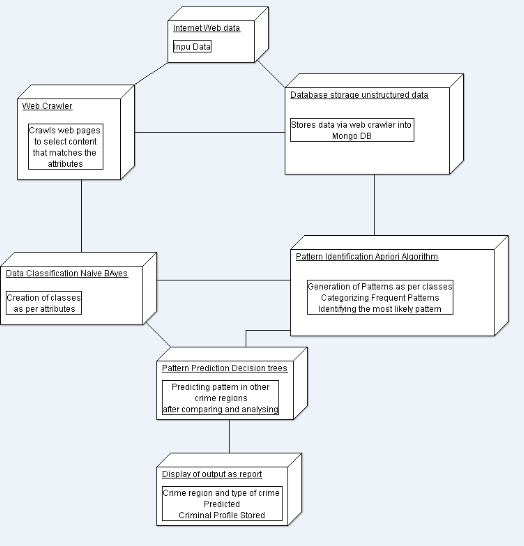
\includegraphics[scale=0.75]{DEPLOYDIAGRAM.png}\\
  \caption{Deployment Diagram}
  \end{figure}
  \pagebreak  
    \subsection{ACTIVITY DIAGRAM}
    \begin{figure}[H]
  \centering
  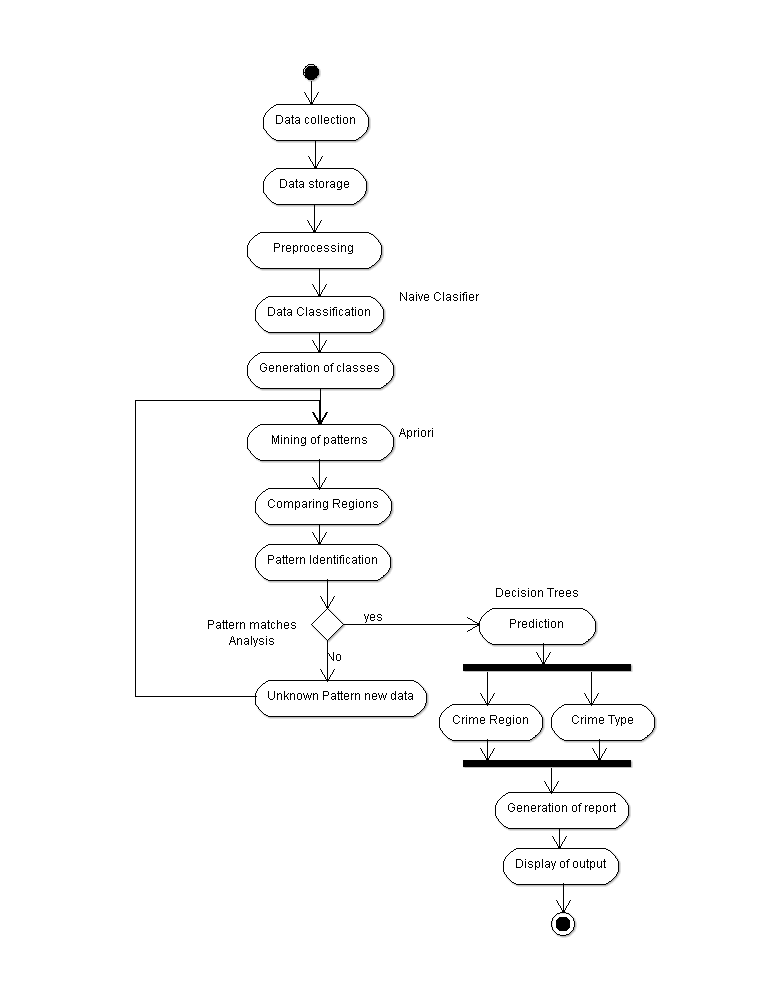
\includegraphics[scale=0.75]{ACTIVITYDIAGCRIME.png}\\
  \caption{Activity Diagram}
  
\end{figure}
    
   \pagebreak 
    \subsection{SEQUENCE DIAGRAM}
    \begin{figure}[H]
  \centering
  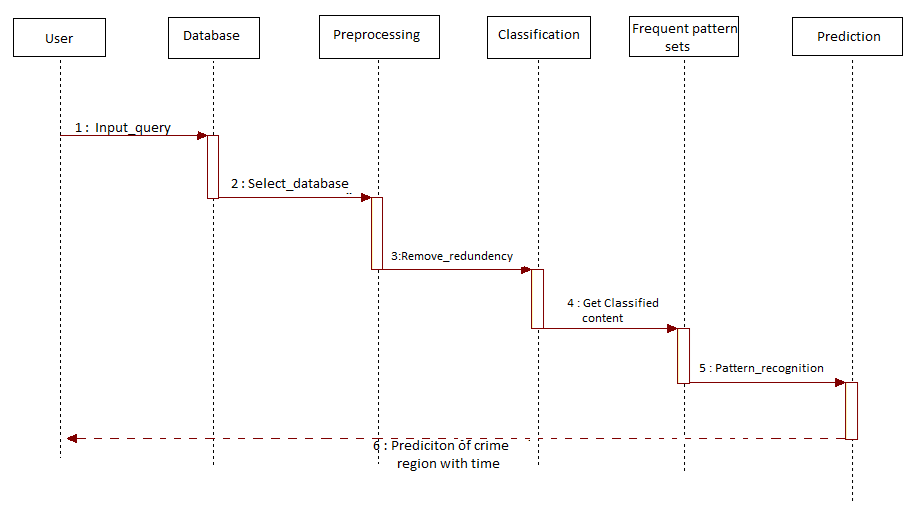
\includegraphics[scale=0.65]{SEQU.png}\\
  \caption{Sequence Diagram}
  
\end{figure}
 \pagebreak   
    \subsection{STATE CHART DIAGRAM}
    
    \begin{figure}[H]
  \centering
  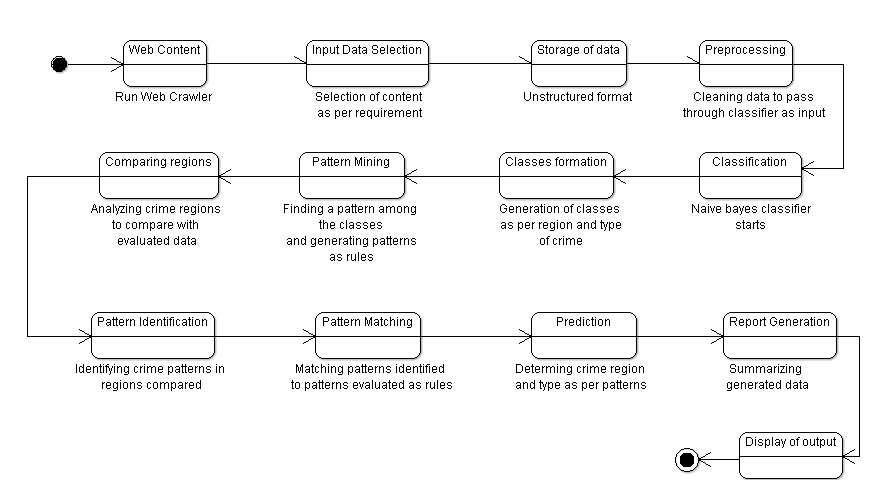
\includegraphics[scale=0.7]{STATECHARTCRIME.png}\\
  \caption{State Chart Diagram}
  
\end{figure}
\pagebreak
    \subsection{CLASS DIAGRAM}
    \begin{figure}[H]
    \centering
  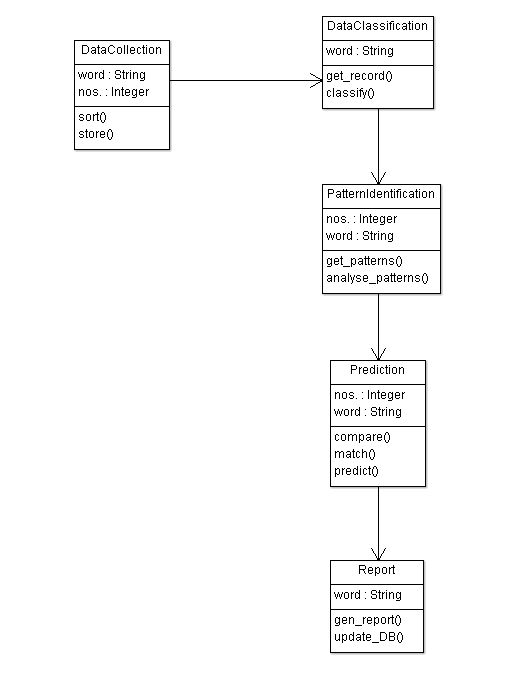
\includegraphics[scale=0.75]{CLASS.png}\\
  \caption{Class Diagram}
  
\end{figure}
%%%%%%%%%%%%%%%%%% CHAPTER 5 %%%%%%%%%%%%%%%%%%%%%%
\chapter{TECHNICAL SPECIFICATION}

\section{ADVANTAGES}
\begin{itemize}
\item User Friendly.
\item Access to authorized personnel only.
\item Memory space utilized efficiently.
\item Multiple algorithms working together to produce best results.

\end{itemize}
 \section{DISADVANTAGES}
\begin{itemize}
 \item May give variable accuracy.
 \item Depending on crime data collected may result in new pattern discovery on each iteration.
 \item Redundant data may exist on multiple iterations.
 \item Crawler may be unable to intercept sufficient amount of data.
\end{itemize} 
 \section{APPLICATIONS}
\begin{itemize}
\item Generates criminal profile and crime patterns.
\item Useful in identifying crime type and matching it to regions more efficiently.
\item Digitized and fast crime analyser.
\end{itemize}

%%%%%%%%%%%%%%%%%% CHAPTER 6 %%%%%%%%%%%%%%%%%%%%%%%
\chapter{RESULTS}
\section{EXPECTED RESULTS}
\hspace*{5em}The application will be able to analyse the crime data from various different internet sources and help in determining a pattern among the crimes occurred in various regions thereby predicting future crime regions and type of crime in these regions also it may help law enforcers to generate criminal profile as per the crime type and region.The system will speed-up the crime analysis process and digitize it so that multiple organizations can benefit from this system at the same time.Such a system may help the law enforcers to reduce crime by deploying resources effectively and preventing criminals from committing crimes thereby providing security to citizens.

\chapter{CONCLUSION}
\hspace*{5em}The existing system consists of 5 phases like Data Collection, Data Classification, Pattern Identification, Prediction and Visualization.The final output of this system is in the form of visuals but the final output of the proposed system is in the form of report so that it can be further analysed and reformed in future by a more improved system than the proposed system.\\

Thus, on the basis of literature survey and by analysing the existing system, we have came to a conclusion that the proposed system will not only aid the law-enforcement agencies but will also help to digitize the criminal database  and in turn help to deploy resources efficiently to prevent crime and increase safety and security of the citizens.


\renewcommand{\bibname}{REFERENCES}
\begin{thebibliography}{11}
\bibitem{DE} Shiju Sathyadevan, Devan M.S and Surya Gangadharan. S., \lq\lq Crime Analysis and Prediction Using Data Mining", Published in 2014 First International Conference on Networks \& Soft Computing, ISBN - 978-1-4799-3486-7 114-2014 IEEE 
\bibitem {} Isuru Jayaweera, Chamath Sajeewa, Sampath Liyanage, Tharindu Wijewardane, Indika Perera and Adeesha Wijayasiri, \lq\lq Crime Analytics: Analysis of Crimes Through Newspaper Articles", ISBN - 978-1-4799-1740-2/15 2015 IEEE

\bibitem {} Hsinchun Chen Wingyan Chung Jennifer Jie Xu Gang Wang Yi Qin and Michael Chau,\lq\lq Crime Data Mining: A General Framework and Some Examples", Published by the IEEE Computer Society ,ISBN - 0018-9162/04/2004 IEEE
\bibitem{} GU Yunhua, SHEN Shu, ZHENG Guansheng,\lq\lq Application of NoSQL Database in Web Crawling", International Journal of Digital Content Technology and its Applications. Volume 5, Number 6, June 2011.
\bibitem {} S.L. Ting, W.H. Ip, Albert H.C. Tsang, \lq\lq Is Naive Bayes a Good Classifier for Document Classification?", International Journal of Software Engineering and Its Applications Vol. 5, No. 3, July, 2013.
\bibitem {} Anagha R Kulkarni, Vrinda Tokekar, Parag Kulkarni,\lq\lq Identifying Context of Text Documents using Naive Bayes Classification and Apriori Association Rule Mining",IET, Devi Ahilya University, Khandawa Road, Indore 452017, India cEKlat Research, Pune, India.
\bibitem{} Mohammed Al-Maolegi1, Bassam Arkok, \lq\lq AN IMPROVED APRIORI ALGORITHM FOR ASSOCIATION RULES",Published in International Journal on Natural Language Computing (IJNLC) Vol. 3, No.1, February 2014.
\bibitem{} Wei Peng, Juhua Chen and Haiping Zhou,\lq\lq An Implementation of ID3 - Decision Tree Learning Algorithm" Project of Comp 9417: Machine Learning University of New South Wales, School of Computer Science\& Engineering, Sydney, NSW 2032, Australia.
\end{thebibliography}

\newpage
\appendix
\chapter{GLOSSARY}
\begin{table}[ht]
\centering
\begin{tabular}{ |p{3cm}|p{8cm}|  }
 \hline
\textbf{STT}& Speech-to-Text \\
\hline
\textbf{TTS} & Text-to-Speech\\
\hline
\textbf{NLTK}&  Natural language toolkit\\
\hline
\textbf{API} & Application Programming Interface\\
\hline
\textbf{JDK} & Java Development Kit\\
\hline
\textbf{GUI} & Graphical User Interface\\
\hline
\textbf{UML} & Unified Modelling Language\\
\hline
\textbf{DB}&  DataBase\\
\hline
\textbf{IOT}&  Internet Of Things\\
\hline
\textbf{LED}&  Light Emitting Diode\\
\hline
\textbf{XML}&  Extensible Markup Language\\
\hline
\textbf{IPA}&  Intelligent Personal Assistant\\
\hline
\textbf{ASR}&  Automatic Speech Recognition\\
\hline






\end{tabular}

\end{table}


\chapter{ASSIGNMENTS}
\section*{\centering\LARGE{Lab Assignment 01}}

\subsection*{\underline{Aim}}
Refer Chapter 7 of first reference to develop the problem under consideration and justify feasibility using concepts of knowledge canvas and IDEA Matrix. 
\subsection*{\underline{Project}}
Crime Analysis and Prediction as an Application of Data Mining.\\

\begin{table}[ht]
\caption{Project Canvas}
\begin{tabular}{ |p{5cm}|p{5cm}|p{5cm}|  }
 \hline
 \textbf{Purpose} & \textbf{Goals} & \textbf{Users}\\
 \hline
To increase safety\& security & To predict crime region \& type& Law-enforcement agencies\\

 
 To reduce crime rate & To digitize criminal data & Crime Analysts\\
 
 \hline

  

 
 \end{tabular}
 
\vspace{0.5cm} 
 
\begin{tabular}{ |p{5cm}|p{5cm}|p{5cm}|  }
 \hline
 \textbf{Actions} & \textbf{Deliverables} & \textbf{Risks} \\
 \hline
 Collect crime data & SRS \& Project Design & DB corruption leads to system error\\


  Analyze collected data & Project Report \& Project & DB may get compromised\\
   \hline
 
 \end{tabular}
 
\vspace{0.5cm} 

 \begin{tabular}{ |p{5cm}|p{5cm}|p{5cm}|  }
 \hline
 \textbf{Milestones} & \textbf{Constraints} & \textbf{Scope} \\
 \hline
 Synopsis, Abstract, Report & Input to be stored in DB & Concurrent Processing\\

  Coding and Final Software  & Software must meet minimum system requirement & Limited to burglary \& pickpocketing\\ 
   \hline
 
 \end{tabular}
  
 
\end{table} 



 
\newpage
\section*{\centering\LARGE{Lab Assignment 02}}
\subsection*{\underline{Aim}}
Project problem statement feasibility assessment using NP-Hard, NP-Complete or satisfy ability issues using modern algebra and/or relevant mathematical models.

\subsection*{\underline{Feasibility Theory}}
The feasibility of the project can be defined as the measure of our project whether it is viable or not.It includes various different types of feasibility as follows:
\begin{itemize}
\item \textbf{Performance:}\\
In this we check whether the proposed system is capable of performing all the functional requirements as mentioned in system features in SRS.If our system is displaying the functional requirements appropriately then it's performance is feasible.Here we also check the accuracy and efficiency of the system based on their algorithms.
\item \textbf{Technical:}\\
In this we check whether the technical specification provided that is hardware and software requirements are minimum requirements for our application software to run successfully without any error regarding the system configuration.Also the  storage requirements is quite enough and concurrency takes place effectively.
\item \textbf{Economical:}\\
In this we check the cost per line of code also the cost for storage of data and cost related to the run time of the system.Apart from this since no extra hardware is needed apart from minimum system configuration for the computers on network.


\end{itemize}
\noindent
\subsection*{\underline{Feasibility on basis of Class of Problem}}
\hspace{5em}Complexity classes are one way to talk about how difficult or easy a problem is.
Complexity theory gets very technical but the basics are actually extraordinarily
intuitive, and it's possible to understand the P versus NP issue with very little
math background.\\

\hspace{1em}If there is a fast solution to the search version of a problem then the problem is
said to be Polynomial time,
or P for short. If there is a fast solution to the verification version of a problem then the problem is said to be
Non deterministic Polynomial time,
or NP for short. The question of
"P=NP" is then the question of whether these sets are identical.\\

\hspace{1em}Some problems can be translated into one another in such a way that a fast
solution to one problem would automatically give us a fast solution to the
other. There are some problems that every single problem in NP can be
translated into, and a fast solution to such a problem would automatically give
us a fast solution to every problem in NP. This group of problems are known as
NP Hard.Some problems in NP Hard
are actually not themselves in NP; the
group of problems that are in both NP and NP Hard
is called NP Complete

\subsection*{\underline{Classes of problems}}
\begin{itemize}
\item \textbf{NP}\\
A lot of programs that don't (necessarily) run in polynomial time
on a regular computer, but do run in polynomial time on a non deterministic
Turing machine. These programs solve problems in NP, which stands for
non deterministic polynomial time.An equivalent way to define NP is by pointing to the problems that can be
verified in polynomial time.

\item \textbf{NP Hard}\\
If a problem is NP hard,
this means I can reduce any problem in NP to that problem. This means if I can solve that problem, I can easily solve any problem in NP. If we could solve an NP hard
problem in polynomial time, this would
prove P = NP.

\item \textbf{NP Complete}\\
A problem is NP complete
if the problem is both
NP hard, and in NP
\end{itemize}

\noindent
\hspace{5em}Since our system satisfies both problems of searching a crime type class and region as well as we are verifying the type of class and region by predicting to find whether pattern of region A matches to pattern in region B.\\

\hspace{1em}Since we have a fast solution to search problem in our project it is said to be P type problem capable to solve a part in polynomial time also the verification version doesn't has a fast solution so it  is not a NP complete problem.
\subsection*{\underline{Relation Between Classes of Problems}}
 \begin{figure}[H]
    \centering
  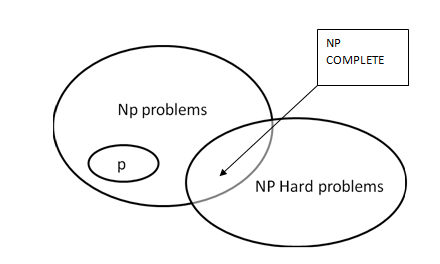
\includegraphics[scale=0.9]{np.png}\\
  \caption{Relation between Classes of Problems}
  
\end{figure}
\subsection*{\underline{Mathematical Model}}
 Let the proposed system be defined by set theory as:\\\\
S= $\{CLA , DC , PRED , PI , S , F , O , I , Q , q_0 , q_f , NDD , D , ALGO \}$ \\ \\
Where, \\ \\
I = input : $\{$ articles, news data, web news data$\}$ \\ \\
O = output :$\{ $type of crime and region as a tuple data$\}$ \\\\
$q_0$ = initial state: $\{$system starts and displays login screen$\}$ \\\\
$q_f$ = final state: $\{$system displays the expected output to user$\}$ \\\\
S = success :$\{$ If the system works accurately without any halt or error.$\}$ \\\\
F = failure :$\{$System halts due to some error or doesn't predict accurately.$\}$\\\\
Q = set of states:$ \{q_0, q_1, q_2, q_3, q_4, q_f\} $\\\\
D = deterministic data : $\{ Null\}$ \\\\
NDD = non deterministic data :$\{$ All states resulting output is non deterministic$\}$\\\\
CLA = classification : $\{ q_2:$ results in classified states or attributes of classes. $\}$\\\\
DC = data collection :$\{ q_1:$ results in data stored in Mongo Db $\}$\\\\
PRED = prediction: $\{q_4:$ results in expected output$\}$\\\\
PI = pattern identification :$\{ q_3:$ results in patterns as association rules$\}$ \\\\
\noindent
\textbf{Naive Bayes Time Complexity : }\\

The complexity of computing the parameters is  
$\Theta(\mid C \mid \mid V\mid)$ because the set of parameters consists of $\mid C \mid \mid V\mid$ conditional probabilities and $\mid C \mid$ priors. The preprocessing necessary for computing the parameters (extracting the vocabulary, counting terms, etc.) can be done in one pass through the training data. The time complexity of this component is therefore $\Theta(\mid D \mid L_{ave})$, where $\mid D \mid$ is the number of documents and $ L_{ave}$ is the average length of a document.\\


\textit{Table 3.1} summarizes the time complexities. In general, we have\\
 $\mid C \mid \mid V\mid < \mid D \mid L_{ave}$, so both training and testing complexity are linear in the time it takes to scan the data.  $ L_{a}$ and $ M_{a}$ are the numbers of tokens and types, respectively. Because we have to look at the data at least once, NB can be said to have optimal time complexity. Its efficiency is one reason why NB is a popular text classification method.\\

\begin{table}[ht]
\caption{Training \& Testing times for Naive Bayes}
\centering
\begin{tabular}{ |M{4cm}|p{7cm}|  }
 \hline
 mode & time complexity \\
 \hline
 training & $\Theta(\mid D \mid L_{ave} + \mid C \mid \mid V \mid)$\\
 \hline 
 testing & $\Theta(L_{a} + \mid C \mid M_a)=\Theta(\mid C \mid M_a)$\\
 \hline
 
 \end{tabular}

\end{table}
\vspace*{1cm}
\noindent
\textbf{Apriori Algorithm Time Complexity:}\\

Suppose the number of input transactions is N, the threshold is M, number of unique elements is R. The complexity for generating set of size i is $O(R\textsuperscript{$\wedge$}i)$ and the time for calculating support for each set can be done in O(n), if using HashMap. Therefore,  time complexity would be\\
\begin{center}
$O[(R + N) + (R\textsuperscript{$\wedge$}2 + N)  + (R\textsuperscript{$\wedge$}3 + N)  …] $\\
$= O[MN + (R\textsuperscript{$\wedge$}1+R\textsuperscript{$\wedge$}2+ … R\textsuperscript{$\wedge$}M)] $\\
$= O(MN+ (1-R\textsuperscript{$\wedge$}M)/(1-R))$
\end{center}



\newpage
\section*{\centering\LARGE{Lab Assignment 03}}
\subsection*{\underline{Aim}}
Use of divide and conquer strategies to exploit distributed/parallel/concurrent processing of the above to identify objects, morphisms, overloading in functions (if any), and functional relations and any other dependencies (as per requirements).
\subsection*{\underline{Concept}}
A divide and conquer algorithm works by recursively breaking down a problem into two or more sub-problems of the same (or related) type (divide), until these become simple enough to be solved directly (conquer). So have divided our problem based on algorithm used and those are:
\begin{itemize}
\item Data Collection.
\item Naive Bayes classifier for classifying (parallel computing used for calculating individual probabilities of the attributes).
\item Apriori algorithm for frequent pattern sets.
\item Decision tree for pattern identification.
\end{itemize}

\vspace*{0.4cm}
\noindent
\hspace{5em}Divide and conquer (D\&C) is an algorithm design paradigm based on multi-branched recursion. So we have to recursively divide our problem into  sub-problems  of the same (or related) type (divide), until these sub-problem become simple enough to be solved directly (conquer). The solutions to the sub-problems are then combined to give a solution to the original problem.\\

\vspace*{0.4cm}
\noindent
\hspace{5em}In our project we have divided our project into 4 phases which are : Data Collection, Data Classification, Pattern identification, and prediction. Now, in Data collection the data is stored as input for next step using a web crawler in a NOSQL database-MongoDB. Further for classifying data Naive Bayes classifier is used which classifies the crime type and its region of interest. Here parallelism will be used where  calculating the probabilities of Each and every class and attribute will be done in parallel.The classified classes are again stored in database and are used as input for next step. Next will be generating frequent pattern sets from the classified data Apriori algorithm. The last step will be generating patterns using decision tree.

\newpage
\noindent
\textbf{System Specifications and Dependencies}\\
The system comprises of following major components : 
\begin{itemize}


\item Data Collection using web crawler.
\item Data Classification using Naive Bayes classifier.
\item Generating frequent pattern sets using apriori algorithm.
\item Pattern identification using decision trees.
\end{itemize}

 \begin{figure}[H]
    \centering
  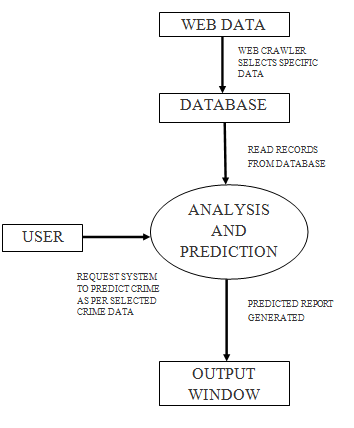
\includegraphics[scale=1.3]{DFDONE.png}\\
  \caption{DFD Level 1}
  
\end{figure}

    \begin{figure}[H]
    \centering
  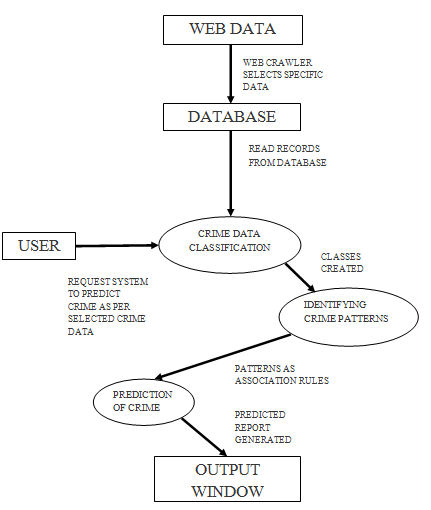
\includegraphics[scale=1.2]{DFDTWO.png}\\
  \caption{DFD Level 2}
  
\end{figure}
\newpage
\section*{\centering\LARGE{Lab Assignment 04}}
\subsection*{\underline{Aim}}
Use of above to draw functional dependency graphs and relevant Software modelling methods, techniques including UML diagrams or other necessities using appropriate tools.
    \subsection*{USE CASE DIAGRAM}
    \begin{figure}[H]
    \centering
  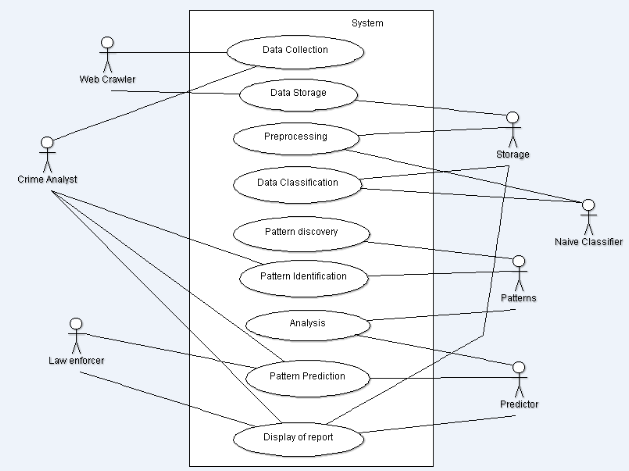
\includegraphics[scale=0.75]{USECRIME.png}\\
  \caption{Use Case Diagram}
  
\end{figure}
    \pagebreak
    \subsection*{DEPLOYMENT DIAGRAM}
     \begin{figure}[H]
  \centering
  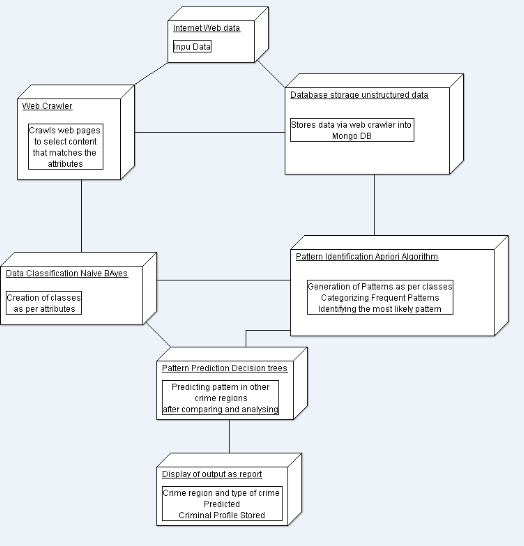
\includegraphics[scale=0.75]{DEPLOYDIAGRAM.png}\\
  \caption{Deployment Diagram}
  \end{figure}
  \pagebreak  
    \subsection*{ACTIVITY DIAGRAM}
    \begin{figure}[H]
  \centering
  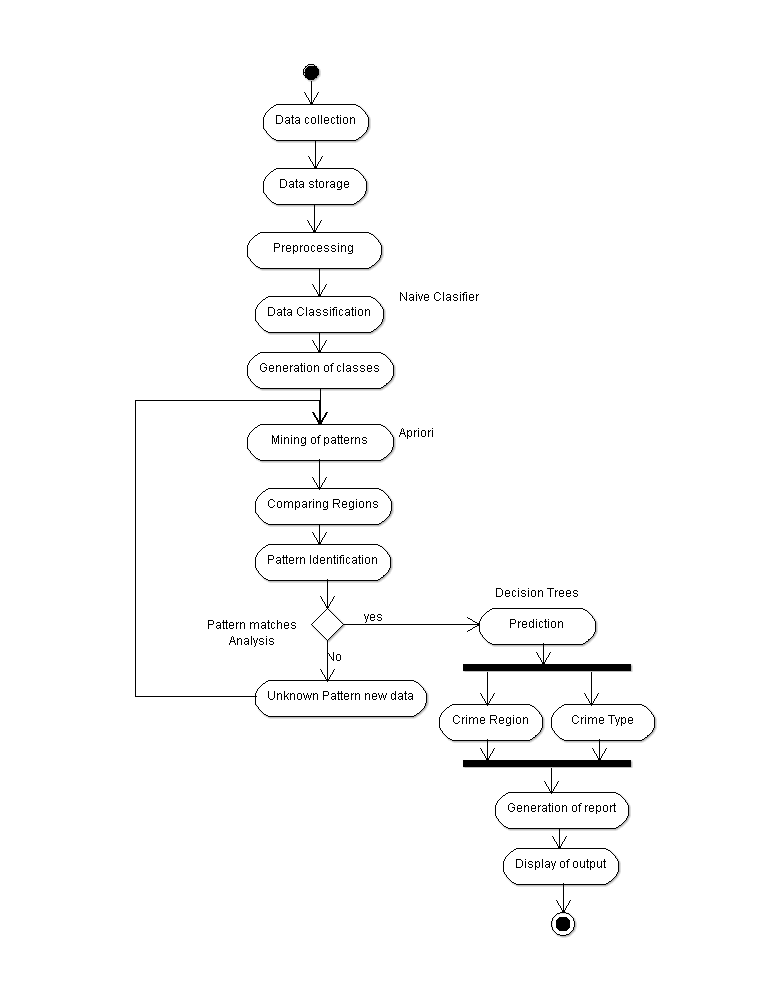
\includegraphics[scale=0.75]{ACTIVITYDIAGCRIME.png}\\
  \caption{Activity Diagram}
  
\end{figure}
    
   \pagebreak 
    \subsection*{SEQUENCE DIAGRAM}
    
    \begin{figure}[H]
  \centering
  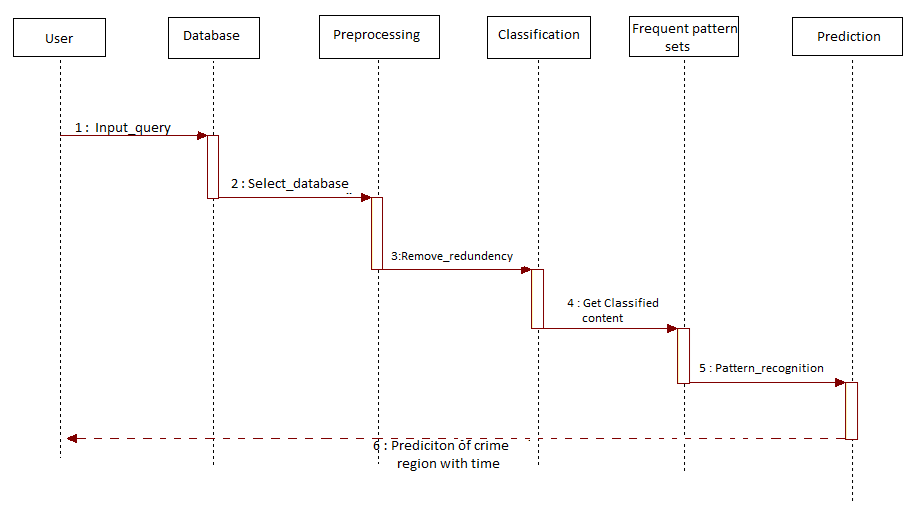
\includegraphics[scale=0.65]{SEQU.png}\\
  \caption{Sequence Diagram}
  
\end{figure}
 \pagebreak   
    \subsection*{STATE CHART DIAGRAM}
    
    \begin{figure}[H]
  \centering
  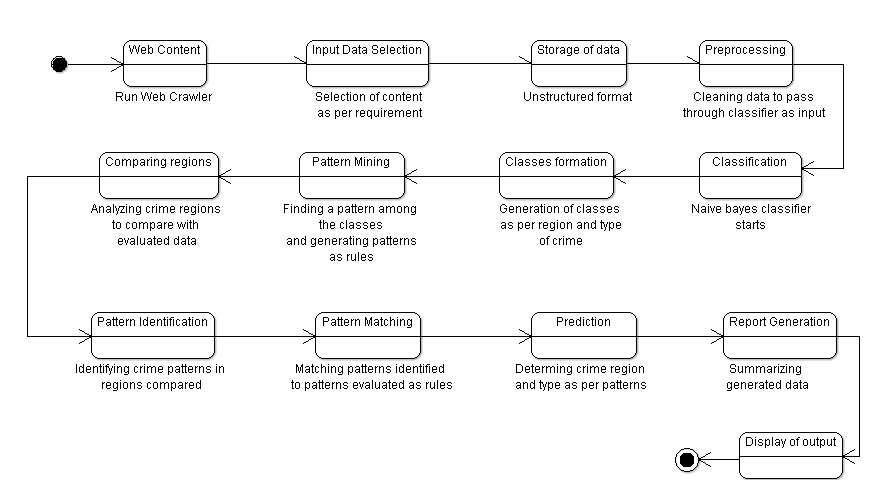
\includegraphics[scale=0.7]{STATECHARTCRIME.png}\\
  \caption{State Chart Diagram}
  
\end{figure}
\pagebreak
    \subsection*{CLASS DIAGRAM}
    \begin{figure}[H]
    \centering
  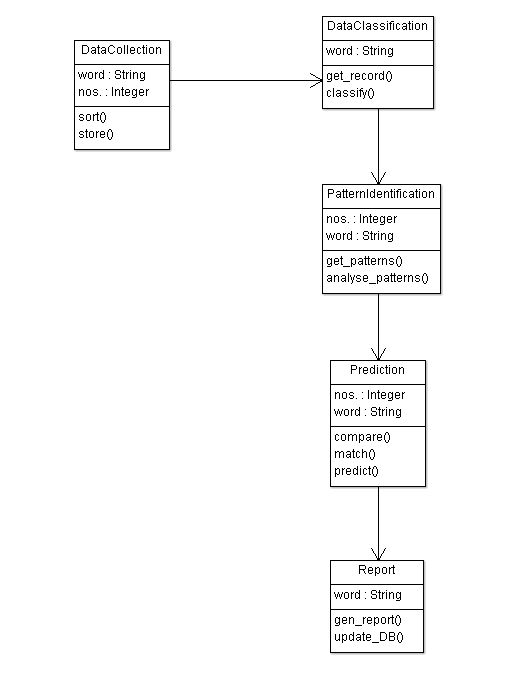
\includegraphics[scale=0.75]{CLASS.png}\\
  \caption{Class Diagram}
  
\end{figure}

\newpage
\section*{\centering\LARGE{Lab Assignment 05}}
\subsection*{\underline{Aim}}
Testing of project problem statement using generated test data (using mathematical models, GUI, Function testing principles, if any) selection and appropriate use of testing tools, testing of UML diagram's reliability.
\noindent
\subsection*{\underline{Testing}}
\hspace{5em}Testing is an investigation conducted to provide stakeholders with information about the quality of the product or service under test. Software testing also provides an objective, independent view of the software to allow the business to appreciate and understand the risks of software implementation. Test techniques include, but are not limited to, the process of executing a program or application with the intent of finding software bugs. Software testing can also be stated as the process of validating and verifying that a software program or application or product.\\

\noindent
\hspace{5em}Software testing, depending on the testing method employed, can be implemented at any time in the development process. However, most of the test effort occurs after the requirements have been defined and the coding process has been completed. As such, the methodology of the test is governed by the software development methodology adopted.In a more traditional model, most of the test execution occurs after the requirements have been defined and the coding process has been completed.


\subsection*{\underline{Testing types}}
It describes which testing types we might follow in our testing life cycle. Here we are using:
\begin{itemize}
\item \textbf{Black Box Testing}\\
Black box testing methods focus on the functional requirements in the software. That is, black box testing enables us to derive sets of input conditions that will fully exercise.\\
All functional requirements of the program Black box testing attempts to find errors in the following categories:
\begin{itemize}
\item Incorrect or missing function
\item	Interface errors
\item	Errors in data structure or external job access
\item	Performance errors
\item	Initialization and termination errors.
 
\end{itemize}

In the proposed application with the help of this technique, we do not use the code to determine a test suite; rather, knowing the problem that we are trying to solve, we come up with four types of test data: 
\begin{enumerate}
\item	Easy-to-compute data,
\item	Typical data,
\item	Boundary / extreme data,
\item	Bogus data.

\end{enumerate}
But in our application we does not provide any external data, the role of user is only to give number of nodes for formation of clusters and for the formation of sink node.


\item \textbf{White Box Testing}\\
White box testing is a set case design method that uses the control structure of the procedural design to derive test cases. Using white box testing methods, we can derive test cases that:
\begin{itemize}
\item 	Guarantee that all independent paths within a module have been exercised at least once.
\item	Exercise all logical decisions on their true and false sides.
\item	Execute all loops at their boundaries and within their operational bounds.
\item	Exercise internal data structures to ensure their validity.

\end{itemize}
In the proposed application the white box testing is done by the us on the implemented code, we study the code and then determines all legal (valid and invalid) and illegal inputs and verifies the outputs against the expected outcomes, which is also determined by studying the implementation code.


\item \textbf{Unit Testing}\\
Unit testing enables a programmer to detect error in coding. A unit test focuses verification of the smallest unit of software design. This testing was carried out during the coding itself. In this testing step, each module going to be work satisfactorily as the expected output from the module.
The front end design consists of various forms. They were tested for data acceptance. Similarly, the back-end also tested for successful acceptance and retrieval of data. The unit testing is done on the developed code. Mainly the unit testing is done on modules.

\item \textbf{System Testing}\\
After performing the integration testing, the next step is output testing of the proposed system. No system could be useful if it doesn't produce the required output in a specified format. The outputs generated are displayed by the user. Here the output format is considered in to two ways. One in on screen and other in printed format.


\item \textbf{Integration Testing}\\
Through each program work individually, they should work after linking together. This is referred to as interfacing. Data may be lost across the interface; one module can have adverse effect on the other subroutines after linking may not do the desired function expected by the main routine. Integration testing is the systematic technique for constructing the program structure while at the same time conducting test to uncover errors associated with the interface. Using integrated test plan prepared in the design phase of the system development as a guide, the integration test was carried out. All the errors found in the system were corrected for the next testing step.
\item \textbf{Functional Testing}

\item \textbf{GUI Testing}

\end{itemize}

\begin{table}[ht]
\caption{Test Cases}
\begin{tabular}{ |M{4cm}|p{5cm}|M{2.5cm}|M{3.2cm}|  }
 \hline
 \textbf{USE CASE} & \textbf{FUNCTION BEING TESTED} & \textbf{INPUT} & \textbf{EXPECTED OUTPUT}\\
 \hline
 
Data Collection & Is data collected properly? & Web data & Stored records in DB\\

\hline
 Data Classification & Is data classified into  classes as per attributes? & Data in DB & Classes of attributes\\
 
 \hline
 Pattern identification & Is unique patterns generated? & Classes from classifier & Patterns as rules.\\
 
 \hline
 Prediction & Is regions having a common pattern? & Rules from apriori & Expected output\\
  
  \hline
  
 
 \end{tabular}
 
\end{table}





\end{document}